\documentclass[11pt,wide]{mwart}
\usepackage[utf8]{inputenc} 
\usepackage[OT4,plmath]{polski}
\usepackage{graphicx}
\usepackage{caption}
\usepackage{subcaption}
\usepackage{epstopdf}
\usepackage{alltt}
\usepackage[section]{placeins}
\usepackage{graphicx}

\usepackage{amsmath,amssymb,amsfonts,amsthm,mathtools}


\usepackage{bbm}
\usepackage{hyperref}
\usepackage{url}

\usepackage{comment}

\date{Wrocław, \today}
\title{\LARGE\textbf{Pracownia z analizy numerycznej}
  \\Sprawozdanie do zadania \textbf{P1.16.}}

\author{Maciej Buszka}

\newtheorem{tw}{Twierdzenie}
\newtheorem{alg}{Algorytm}

\begin{document}
\maketitle

\section{Wstęp}

Problem rozwiązania układu równań nieliniowych jest często napotykany w fizyce, matematyce i informatyce, wiele innych problemów można także zredukować do znalezienia pierwiastków układu równań nieliniowych. W tym sprawozdaniu opiszę metodę Newtona, czyli iteracyjny algorytm znajdujący pierwiastek funkcji $ F : \mathbb{R}^n \rightarrow \mathbb{R}^n $, czyli rozwiązanie równania $ F(X) = 0 $. Na podstawie różnych testów numerycznych zbadam zbieżność oraz zachowanie tej metody dla małych i dużych układów równań liniowych.
\section{Metoda Newtona}
\subsection{Intuicja i opis}

Dla funkcji jednej zmiennej $ f(x) = y $ metoda Newtona opiera się na założeniu że w okolicach punktu $ x_n $ możemy przybliżyć funkcję $ f $ funkcją liniową $ l(x) = f'(x_n)(x - x_n) + f(x_n) $. Można łatwo przekształcić ten wzór tak aby znaleźć miejsce zerowe tej funkcji liniowej.

\begin{equation} \label{eq:newtonsimple}
		x_{n+1} = x_n - \frac{f(x_n)}{f'(x_n)}
\end{equation}

Otrzymaną zależność możemy zinterpretować następująco: jeżeli $ x_n $ jest wystarczająco blisko miejsca zerowego $ \alpha $ funkcji $ f $, to chcielibyśmy znaleźć taką poprawkę $ h $ aby $ f(x_n + h) = f(\alpha) = 0 $. Korzystając ze wzoru Taylora $ f(x_n + h) = f(x_n) + f'(x_n)h + \dots $ zakładając, że $ x_n $ jest blisko $ \alpha $ otrzymujemy równanie $ h = -\frac{f(x_n)}{f'(x_n)} $. Zatem z równania \eqref{eq:newtonsimple} $ f(x_{n+1}) \approx 0 $ co pokazuje, że taka zależność może dać nam ciąg zbieżny do $ \alpha $.\\
 
Analogiczne rozumowanie chcielibyśmy teraz przeprowadzić dla funkcji $ F : \mathbb{R}^n \to \mathbb{R}^n $. Można ją zapisać w postaci wektora funkcji:

$$ 
F(X) = F(x_1, x_2, \ldots, x_n) = 
\left(\begin{matrix}
	f_1(x_1, x_2, \ldots, x_n) \\ 
	f_2(x_1, x_2, \ldots, x_n) \\ 
	\vdots\\ 
	f_n(x_1, x_2, \ldots, x_n)
\end{matrix}\right)
$$
Jeżeli funkcja $ F $ jest różniczkowalna w punkcie $ X_0 $ to macierz jej pochodnych cząstkowych nazywana Jakobianem jest macierzą przekształcenia liniowego które jest najlepszym przybliżeniem $ F $
$$ J = 
\begin{pmatrix}
\frac{\partial f_1}{\partial x_1} & \frac{\partial f_1}{\partial x_2} &  \ldots & \frac{\partial f_1}{\partial x_n} \\ 

 \vdots & & & \vdots  \\ 
\frac{\partial f_n}{\partial x_1} & \frac{\partial f_n}{\partial x_2} &  \ldots & \frac{\partial f_n}{\partial x_n} \\ 
\end{pmatrix}
$$
Korzystając ze wzoru Taylora dla funkcji $ F $ w punkcie $ X^{(n)} $ chcielibyśmy aby $ H$ było taką poprawką, że $ F(X^{(n)} + H) = 0 $
$$
 	0 = F(X^{(n)} + H) \approx F(X^{(n)}) + J(X^{(n)})H
$$
Stąd
\begin{equation} \label{eq:newtonH}
	J(X^{(n)})H = -F(X^{(n)})
\end{equation}
Jeśli J jest odwracalna, to możemy przekształcić równanie \eqref{eq:newtonH} do postaci
$$ 
	H = -J^{-1}(X^{(n)})F(X^{(n)}) 
$$
I wykorzystać tą zależność do znalezienia następnego przybliżenia miejsca zerowego funkcjji $ F $

\begin{equation} \label{eq:newtonrec}
	X^{(n + 1)} = X^{(n)} + H
\end{equation}
\begin{equation*}
	X^{(n + 1)} = X^{(n)} - J^{-1}(X^{(n)})F(X^{(n)})
\end{equation*}
Niestety aby bezpośrednio wykorzystać powyższe równanie musielibyśmy w każdym kroku  obliczać odwrotność macierzy $ J(X^{(n)}) $ co jest kosztowne. Zamiast tego lepiej bezpośrednio rozwiązać równanie \eqref{eq:newtonH} i otrzymane $ H $ podstawić do wzoru \eqref{eq:newtonrec}

\subsection{Analiza teorytyczna}

Zbieżność metody Newtona dogłębnie analizują J.~C.~Ortega oraz W.~C.~Rheinboldt w \cite{ortega}. Przytoczę tutaj najważniejsze z twierdzeń.
\begin{tw}
Załóżmy, że $ F : D \subset \mathbb{R}^n \rightarrow \mathbb{R}^n $ jest różniczkowalna w otwartym otoczeniu $ S_0 \subset D $ punktu $ x^* $ takiego, że $ F(x^*) = 0 $, $ J = F' $ jest ciągła w $ x^* $ oraz macierz $ J(x^*) $ jest nieosobliwa, to metoda Newtona jest zbieżna nadliniowo dla $ x^{(0)} \in S_0 $. Jeśli ponadto pochodna $ F' $ jest ciągła na $ S_0 $ oraz druga pochodna $ F'' $ istnieje w $ x^* $ oraz 
\begin{align}
	\forall h \in \mathbb{R}^n, h \neq 0 \quad F''(x^*)hh \neq 0
\end{align}
to metoda Newtona jest zbieżna kwadratowo
\end{tw}
\begin{proof}
	Udowodnione w \cite{ortega} str 312-313
\end{proof}
\subsection{Implementacja}
Metodę newtona bardzo łatwo zaimplementować o ile założymy, że Jakobian funkcji jest nam dany. W poniższym algorytmie zakładamy, że przekazane są $ F $ - funkcja, $ J $ - pochodna tej funkcji, $ X $ - przybliżenie początkowe oraz \texttt{eps} i \texttt{imax} -kryteria zatrzymania, odpowiednio tolerowany błąd względny przybliżenia jak i maksymalna liczba iteracji. W algorytmie wykorzystuję funkcję biblioteczną \texttt{norm(X} która oblicza normę wektora $ X $ oraz funkcję \texttt{solve(A, B)} która rozwiązuje układ równań $ AX = B $, która zaimplentowana przeze mnie wykorzystuje metodę eliminacji Gaussa
\begin{verbatim}
		Dane: F, J, X, eps = 1e-15, imax = 20
		Wynik : X
		
		i := 0
		e := 1.0
		while e > eps and i < imax do
		  JX := J(X)
		  FX := F(X)
		  H  := solve(JX, FX)
		  e  := norm(H) / norm(X)
		  X  := X - H
		  i  := i + 1
		done			
\end{verbatim}
\subsection{Koszt iteracji}
W każdej iteracji głównej pętli metody Newtona musimy wykonać następujące kosztowne operacje:
\begin{enumerate}
\item Obliczenie wartości funkcji $ F(X) $
\item Obliczenie wartości jakobianu $ J(X) $
\item Obliczenie normy $ X $ i $ H $
\item Rozwiązanie układu równań $ J(X)H = F(X)$
\end{enumerate}
Koszt dwóch pierwszych nie jest zależny od implementacji metody Newtona, koszt trzeciej jest liniowy względem wielkości wektora $ H $, natomiast koszt rozwiązania układu równań jest zanalizowany w rozdziale \ref{SS:gausscost}
\section{Metoda eliminacji Gaussa}
\subsection{Opis} \label{p:gaussopis}
Metoda eliminacji Gaussa jest najprostszym koncepcyjnie algorytmem rozwiązywania układu równań liniowych postaci $ AX = B $.
Składa się on z dwóch faz: eliminacji i podstawiania. Rozważmy układ
$$
\left(\begin{matrix}
a_{11} & a_{12} & \ldots & a_{1n} \\
a_{21} & a_{22} & \ldots & a_{2n} \\
\vdots & \vdots & 		 & \vdots \\
a_{i1} & a_{i2} & \ldots & a_{in} \\
\vdots & \vdots & 		 & \vdots \\
a_{n1} & a_{n2} & \ldots & a_{nn}
\end{matrix}\right)
\left(\begin{matrix}
x_1 \\ x_2 \\ \vdots \\ x_i \\ \vdots \\ x_n
\end{matrix}\right) = 
\left(\begin{matrix}
b_1 \\ b_2 \\ \vdots \\ b_i \\ \vdots \\ b_n
\end{matrix}\right)
$$
W fazie eliminacji chcemy sprowadzić go do postaci górnotrójkątnej tj.
$$
\left(\begin{matrix}
a_{11} & a_{12} &  & \ldots  & & a_{1n} \\
0 & a_{22} &  & \ldots  & & a_{2n} \\
\vdots & \vdots & \ddots &		 & & \vdots \\
0 & 0 & \ldots & a_{ii}  & \ldots & a_{in} \\
\vdots & \vdots &  &		 & \ddots & \vdots \\
0 & 0 &  & \ldots  & 0 & a_{nn}
\end{matrix}\right)
\left(\begin{matrix}
x_1 \\ x_2 \\ \vdots \\ x_i \\ \vdots \\ x_n
\end{matrix}\right) = 
\left(\begin{matrix}
b_1 \\ b_2 \\ \vdots \\ b_i \\ \vdots \\ b_n
\end{matrix}\right)
$$
Możemy to osiągnąć odejmując odpowiednią wielokrotność pierwszego wiersza od pozostałych, a następnie powtarzając ten krok dla macierzy z obciętym pierwszym wierszem i kolumną. Tak więc w $ k $-tym powtórzeniu procedury musimy wykonać następujące podstawienia:
\begin{equation}
\begin{cases}
	\alpha_k \leftarrow \frac{a_{ik}}{a_{kk}} \\
	a_{ij} \leftarrow a_{ij} - \alpha_k a_{kj} \\
	b_{i} \leftarrow b_{i} - \alpha_k b_{i}
\end{cases} \text{ dla }(k \leq j \leq n), (k + 1 \leq i \leq n)
\end{equation}
Współczynnik $ \alpha_k $ nazywamy mnożnikiem, natomiast wyraz $ a_{kk} $ elementem głównym względem którego redukujemy nasz układ. Gdy już otrzymamy macierz w postaci górnotrójkątnej, wystarczy wykonać podstawienia 
$$ 
\begin{cases}
	x_n \leftarrow \frac{b_n}{a_{nn}} \\
	x_k \leftarrow \frac{b_k - \sum_{j = k+1}^{n} a_{kj}x_{j}}{a_{kk}} \quad \text{ dla } k = (n-1, \ldots ,  1)
\end{cases}
$$
aby otrzymać wynik
\subsection{Znaczenie elementów głównych}
Podczas implementacji metody Gaussa największym problemem jest wybór wiersza względem którego będziemy wykonywać eliminację. Po pierwsze nie może on mieć zerowego elementu głównego. Po drugie, jeżeli będzie on bardzo mały względem innych elementów w tej kolumie macierzy, natrafimy na błędy wynikające z dodawania i odejmowania bardzo dużych liczb. Rozważmy dla przykładu układ równań
\begin{align} \label{eq:gaussfail}
\left(\begin{matrix}
\epsilon & 1	\\
       1 & 1
\end{matrix}\right)
\left(\begin{matrix}
x_1 \\ x_2
\end{matrix}\right) = 
\left(\begin{matrix}
1 \\ 2
\end{matrix}\right)
\end{align}
W pierwszym (i jedynym) kroku eliminacji przekształcony zostanie on do postaci
\begin{align*}
\left(\begin{matrix}
\epsilon & 1	\\
 0 & 1 - \epsilon^{-1}
\end{matrix}\right)
\left(\begin{matrix}
x_1 \\ x_2
\end{matrix}\right) = 
\left(\begin{matrix}
1 \\ 2 - \epsilon^{-1}
\end{matrix}\right)
\end{align*}
Ma on rozwiązania 
$$ 
x_2 = \frac{2 - \epsilon^{-1}}{1 - \epsilon^{-1}} \approx 1 \quad x_1 = \frac{(1 - x_2)}{\epsilon} \approx 1
$$
Jednak przy obliczaniu tych wartości, dla odpowiednio małego $ \epsilon $,  $ 2 - \epsilon^{-1} = 1 - \epsilon^{-1} = \epsilon^{-1} $ co daje nam $ x_2 = 1 $ i $ x_1 = 0 $, co jest absurdalnym wynikiem. Gdyby poprzedni układ zapisać w postaci
\begin{align*}
\left(\begin{matrix}
       1 & 1 \\
\epsilon & 1
\end{matrix}\right)
\left(\begin{matrix}
x_1 \\ x_2
\end{matrix}\right) = 
\left(\begin{matrix}
1 \\ 2
\end{matrix}\right)
\end{align*}
otrzymalibyśmy poprawny wynik, co jest pokazane w \cite{kincaid}
Widzimy zatem, że konieczne jest odpowiednie wybieranie wiersza względem którego wykonamy redukcję.
\subsection{Implementacja}
Wykorzystamy algorytm eliminacji Gaussa ze skalowanym wyborem wierszy głównych opisany w [Kincaid]. Radzi on sobie z zerowymi oraz znacząco różnymi elementami głównymi macierzy permutując na bierząco kolejność wierszy. Na początku tworzymy wektor skal $ s_i = \max_{1 \leq k \leq n}a_{ik} $, po czym w \texttt{k}-tym kroku wybieramy wiersz w którym iloraz $ \frac{a_{kj}}{s_j} (j = k, k+1, \ldots,n)$ jest najmniejszy. Poza tą modyfikacją algorytm jest jak w \S\ref{p:gaussopis} Pseudokod dostępny jest w \cite{kincaid}, a jego implementacja w języku Julia znajduje się w pliku \texttt{gauss.jl}
\subsection{Koszt} \label{SS:gausscost}
\subsection{Wskaźnik uwarunkowania macierzy}
\section{Wyniki eksperymentów}
\subsection{Znaczenie elementu głównego w eliminacji Gaussa}
Porównam tutaj zachowanie naiwnej implementacji eliminacji Gaussa i algorytmu ze skalowanym elementem głównym w arytmetyce podwójnej precyzji (typ danych \texttt{Float64})
\begin{center}
\begin{table}[!htb]
    \begin{subtable}{.5\linewidth}
      \centering
        \caption{naiwna}
\begin{tabular}{| c | c | c |} \hline
$ \epsilon $ & $x_1$ & $x_2$ \\ \hline
1.00000e-01 & 1.1111111e+00 & 8.8888889e-01 \\ 
1.00000e-02 & 1.0101010e+00 & 9.8989899e-01 \\
\vdots & \vdots & \vdots \\
1.00000e-14 & 9.9920072e-01 & 1.0000000e+00 \\ 
1.00000e-15 & 9.9920072e-01 & 1.0000000e+00 \\ 
1.00000e-16 & 0.0000000e+00 & 1.0000000e+00 \\ 
1.00000e-17 & 0.0000000e+00 & 1.0000000e+00 \\
\vdots & \vdots & \vdots \\ \hline
\end{tabular}
\end{subtable}%
\begin{subtable}{.5\linewidth}
\centering
\caption{ze skalowanym elementem głównym}
\begin{tabular}{| c | c | c |} \hline
$ \epsilon $ & $x_1$ & $x_2$ \\ \hline
1.00000e-01 & 1.1111111e+00 & 8.8888889e-01 \\ 
1.00000e-02 & 1.0101010e+00 & 9.8989899e-01 \\ 
\vdots & \vdots & \vdots \\
1.00000e-14 & 1.0000000e+00 & 1.0000000e+00 \\ 
1.00000e-15 & 1.0000000e+00 & 1.0000000e+00 \\ 
1.00000e-16 & 1.0000000e+00 & 1.0000000e+00 \\ 
1.00000e-17 & 1.0000000e+00 & 1.0000000e+00 \\
\vdots & \vdots & \vdots \\ \hline
\end{tabular}
\end{subtable}
\caption{Porównanie implementacji eliminacji Gaussa dla układu \eqref{eq:gaussfail}}
\end{table}
\end{center}
\subsection{Małe układy równań}
Pokazane są tutaj przebiegi metody Newtona dla dwóch funkcji $ F $ i $ G $, a także porównanie tempa zbieżności wszystkich funkcji testowych, których wzory można zobaczyć w zeszycie interaktywnym \texttt{program.ipynb} za pomocą programu \texttt{jupyter}.
\begin{align*}
F(x) = 
\left(\begin{matrix}
	(x_1)^2 + (x_2)^2 - 25 \\
	(x_1)^2 - x_2 - 2
\end{matrix}\right) && G(x) =
\left(\begin{matrix}
(x_1)^3 + 7(x_2)^2 - 7 \\
(x_1)^2 + (x_2)^2 - 1
\end{matrix}\right)
\end{align*}
\begin{center}
\begin{table}[!htb]
    \begin{subtable}{.5\linewidth}
      \centering
      \caption{Zbieżność kwadratowa dla funkcji $ F $}
\begin{tabular}{| c | c | c |} \hline
Iteracja & $\|F(X)\|$ & $\epsilon$ \\ \hline
0 & 3.114482e+01 & 5.884301e+00 \\ 
1 & 5.301945e+01 & 3.675183e-01 \\ 
2 & 9.411666e+00 & 1.725992e-01 \\ 
3 & 7.950828e-01 & 2.592261e-02 \\ 
4 & 1.475216e-02 & 5.889474e-04 \\ 
5 & 8.572156e-06 & 3.413509e-07 \\ 
6 & 2.913225e-12 & 1.158651e-13 \\ 
7 & 1.256074e-15 & 3.663005e-17 \\ \hline
\end{tabular}
      \caption*{Przybliżenie początkowe $ x_0 = (1, 1)^T $}
\end{subtable}%
\begin{subtable}{.5\linewidth}
\centering
\caption{Zbieżność liniowa dla funkcji $ G $}
\begin{tabular}{ |c | c | c| } \hline
Iteracja & $\|F(X)\|$ & $\epsilon$ \\ \hline
0 & 4.472136e+00 & 1.264911e+00 \\ 
1 & 2.031359e+01 & 8.820599e-01 \\ 
2 & 1.371753e+01 & 4.438798e-01 \\
\vdots & \vdots & \vdots \\
14 & 1.599900e-07 & 1.999594e-04 \\ 
15 & 3.998376e-08 & 9.997112e-05 \\ 
16 & 9.994225e-09 & 4.998342e-05 \\ 
17 & 2.498342e-09 & 2.499117e-05 \\ 
18 & 6.245589e-10 & 1.249545e-05 \\ 
19 & 1.561364e-10 & 6.247696e-06 \\ \hline
\end{tabular}
\caption*{Przybliżenie początkowe $ x_0 = (1, 2)^T $}
\end{subtable}
\caption{Porównanie zbieżności metody Newtona}
\end{table}
\end{center}
\begin{figure}[p]
    \centering
    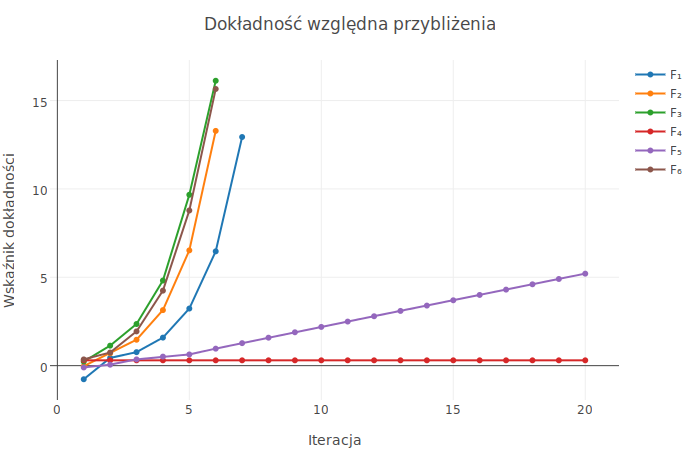
\includegraphics[width=0.8\textwidth]{rel_precision}
    \caption{Porównanie względnej dokładności przybliżenia dla różnych funkcji}
    \label{fig:relprecision}
\end{figure}
\begin{figure}[p]
    \centering
    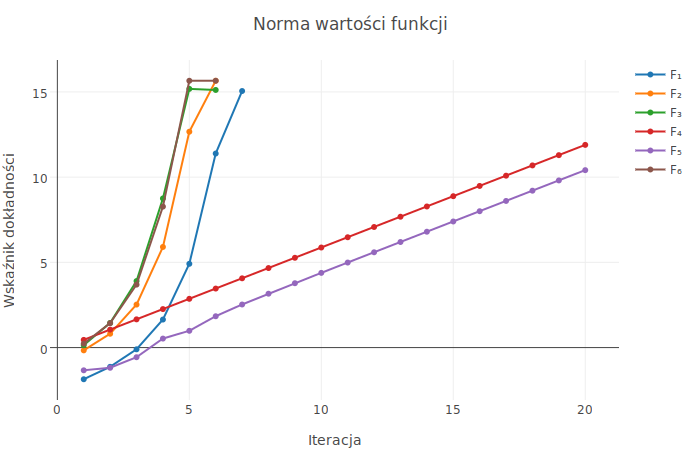
\includegraphics[width=0.8\textwidth]{norm}
    \caption{Porównanie wartości $ \| F(X) \| $ dla różnych funkcji}
    \label{fig:norm}
\end{figure}
Jako wskaźnik dokładności przyjąłem wartość $ y = -\log_{10}\epsilon $ dla błędu względnego oraz $ y = -\log_{10}\|F(X)\| $ dla wartości funkcji
\FloatBarrier
\subsection{Duże układy równań}
Tutaj porównam ilość iteracji metody Newtona potrzebną do znalezienia pierwiastka funkcji o $ n $ niewiadomych. Testy przeprowadzono dla czterech funkcji, dla każdej z nich jednym z miejsc zerowych jest wektor $ \bar{x} = (1, 1, \ldots, 1)^T $, natomiast przybliżenie początkowe to wektor $ x^{(0)} = (x_1, x_2, \ldots, x_n )$ o losowo wybranych współczynnikach $ x_i \in (1-\delta, 1+\delta) $. Zbadałem następujące funkcje
\begin{align}
	F(x) &= 
	\left(\begin{matrix}
		f_1(x) - f_1(\bar{x}) \\ 
		f_2(x) - f_2(\bar{x}) \\ 
		\vdots\\ 
		f_n(x) - f_n(\bar{x})
	\end{matrix}\right), && \text{dla} \quad f_i(X) = a_{ik}X_iX_k, \quad a_{ik} \in (-10, 10) \label{eq:F}\\
	G(x) &=
	\left(\begin{matrix}
	g_1(x) - g_1(\bar{x}) \\ 
	g_2(x) - g_2(\bar{x}) \\ 
	\vdots\\ 
	g_n(x) - g_n(\bar{x})
\end{matrix}\right), && \text{dla} \quad g_i(X) = (x_i)^2\ + \sum_{k=1, k\neq i}^{n}\sin{x_i}cos{x_k} \label{eq:G}\\
	H(x) &= 
	\left(\begin{matrix}
	h_1(x) - h_1(\bar{x}) \\ 
	h_2(x) - h_2(\bar{x}) \\ 
	\vdots\\ 
	h_n(x) - h_n(\bar{x})
\end{matrix}\right), && \text{dla} \quad h_i(X) = 
		\begin{cases}  
			\sin{x_i}\sin{x_{i+1}}\cos{x_{i+2}}, & \text{ gdy } i \leq n-2 \\
			\sin{x_{n-1}}\sin{x_{n}}\cos{x_{1}}, & \text{ gdy } i = n - 1 \\
			\sin{x_n}\sin{x_{1}}\cos{x_{2}}, & \text{ gdy } i = n
		\end{cases} \label{eq:H} \\
	V(x) &=
	\left(\begin{matrix}
		v_1(x) - v_1(\bar{x}) \\ 
		v_2(x) - v_2(\bar{x}) \\ 
		\vdots\\ 
		v_n(x) - v_n(\bar{x})
	\end{matrix}\right), && \text{dla} \quad v_i(x) = x_1 + (i+1)x_2 + \ldots + (i+1)^{n-1}x_n \label{eq:V}
\end{align}
Dla każdej wartości $ n = 2, 3, \ldots, 20 $ i parametru $ \delta = 0.1, 0.2, 0.5, 1.0 $ przeprowadziłem 1000 prób, w których na nowo były losowane wektory początkowe oraz współczynniki $ a_{ik} $ dla funkcji $ F $. Wyniki wszystkich prób dla określonego $ n $ oraz $ \delta $ uśredniłem. Przyjąłem następujące kryteria zatrzymania iteracji:
\begin{itemize}
\item \texttt{maxiter =} $ 5n $ - maksymalna liczba iteracji (powstrzymuje program w przypadku rozbieżności).
\item $ \epsilon_s = 10^{-12} $ - zarówno tolerancja błędu względnego przybliżenia, jak i tolerancja wartości $ \|F(X)\| $.
\end{itemize}
Obliczenia wykonane zostały dla typu danych \texttt{Float64}.
\begin{center}
\begin{table}[!htb]
    \begin{subtable}{.5\linewidth}
      \centering
\begin{tabular}{ |c | c | c| } \hline
Iteracja & $\|F(X)\|$ & $\epsilon$ \\ \hline
0 & 7.113507e+01 & 4.435757e-01 \\ 
1 & 3.587656e+01 & 1.685290e-01 \\ 
2 & 3.579608e+00 & 2.631299e-02 \\ 
3 & 2.296047e-01 & 2.199988e-03 \\ 
4 & 7.829980e-04 & 1.532992e-05 \\ 
5 & 5.522215e-08 & 2.608613e-10 \\ 
6 & 3.436562e-14 & 2.343784e-16 \\  \hline
\end{tabular}
\caption{Funkcja $ F $}
\end{subtable}%
\begin{subtable}{.5\linewidth}
\centering
\begin{tabular}{| c | c | c |} \hline
Iteracja & $\|F(X)\|$ & $\epsilon$ \\ \hline
0 & 1.757268e+01 & 3.069187e-01 \\ 
1 & 1.323588e+01 & 1.108648e-01 \\ 
2 & 3.287417e+00 & 2.735830e-02 \\ 
3 & 2.506188e-01 & 1.954874e-03 \\ 
4 & 1.143128e-03 & 1.026775e-05 \\ 
5 & 3.456163e-08 & 2.875731e-10 \\ 
6 & 2.188678e-14 & 2.533492e-16 \\ \hline
\end{tabular}
\caption{Funkcja $ G $}
\end{subtable}
\caption{Przykładowa iteracja metody Newtona, dla układu rozmiaru $ n = 20 $ }
\end{table}
\end{center}
Badając liczbę iteracji brałem pod uwagę jedynie przebiegi w których metoda była zbieżna.
\begin{figure}[h]
    \centering
    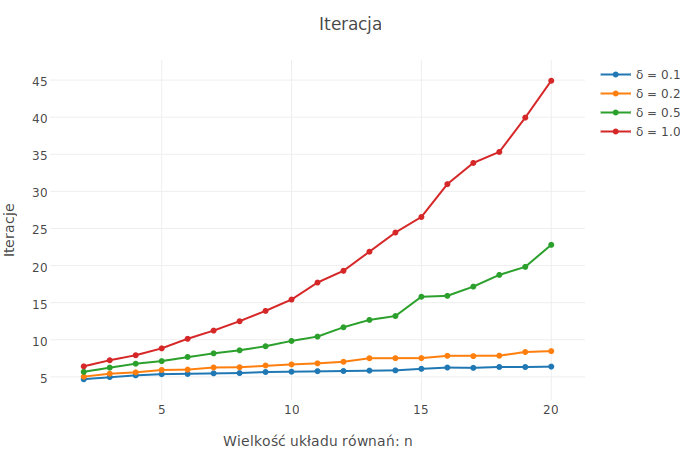
\includegraphics[width=0.9\textwidth]{avg_iterations_F}
    \caption{Średnia ilość iteracji potrzebna do zakończenia metody Newtona dla funkcji F \eqref{eq:F}}
    \label{fig:avgiterationsF}
\end{figure}
\begin{figure}[h]
    \centering
    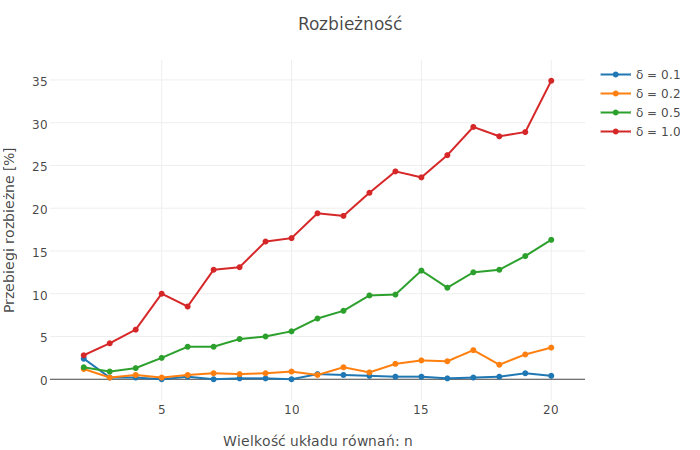
\includegraphics[width=0.9\textwidth]{avg_diversions_F}
    \caption{Procent uruchomień metody Newtona dla funkcji F \eqref{eq:F}, które nie zbiegły w limicie iteracji}
    \label{fig:avgdiversionsF}
\end{figure}
\begin{figure}[h]
    \centering
    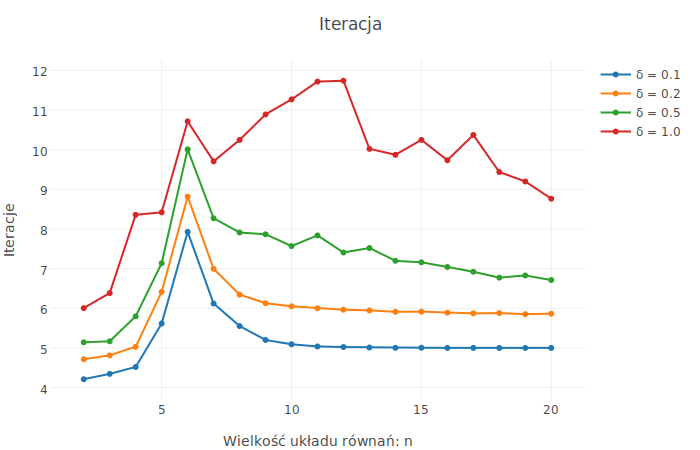
\includegraphics[width=0.9\textwidth]{avg_iterations_G}
    \caption{Średnia ilość iteracji potrzebna do zakończenia metody Newtona dla funkcji G \eqref{eq:G}}
    \label{fig:avgiterationsG}
\end{figure}
\begin{figure}[h]
    \centering
    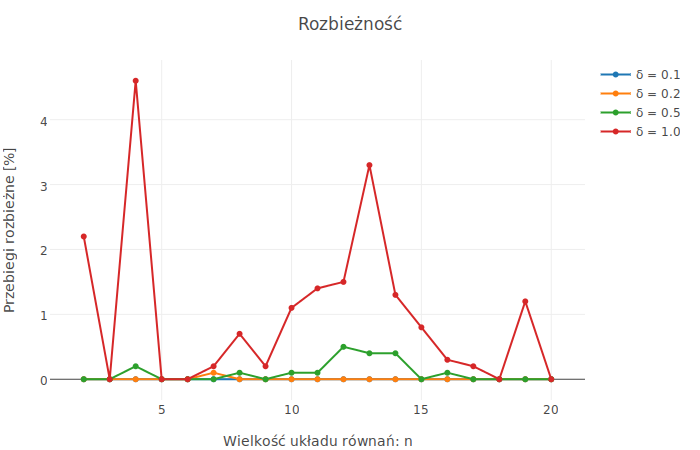
\includegraphics[width=0.9\textwidth]{avg_diversions_G}
    \caption{Procent uruchomień metody Newtona dla funkcji G \eqref{eq:G}, które nie zbiegły w limicie iteracji}
    \label{fig:avgdiversionsG}
\end{figure}
\begin{figure}[h]
    \centering
    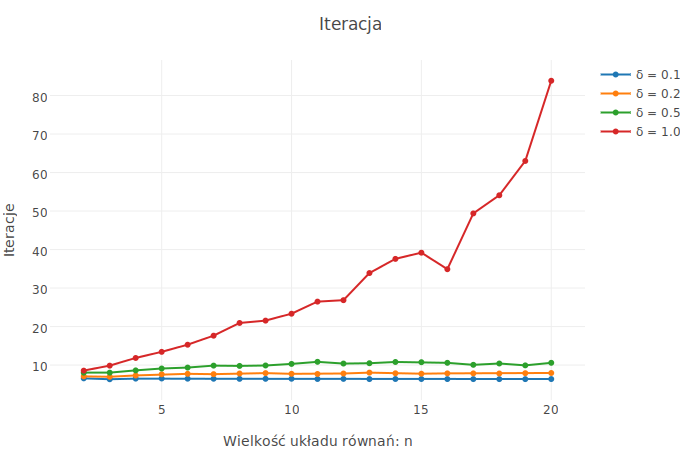
\includegraphics[width=0.9\textwidth]{avg_iterations_H}
    \caption{Średnia ilość iteracji potrzebna do zakończenia metody Newtona dla funkcji H \eqref{eq:H}}
    \label{fig:avgiterationsH}
\end{figure}
\begin{figure}[h]
    \centering
    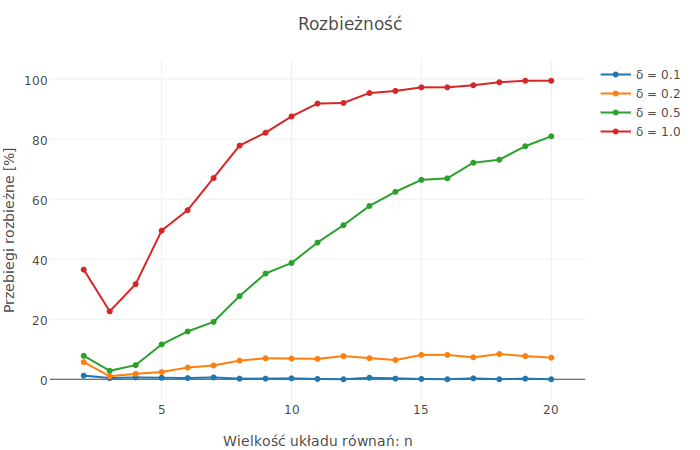
\includegraphics[width=0.9\textwidth]{avg_diversions_H}
    \caption{Procent uruchomień metody Newtona dla funkcji H \eqref{eq:H}, które nie zbiegły w limicie iteracji}
    \label{fig:avgdiversionsH}
\end{figure}
\begin{figure}[h]
    \centering
    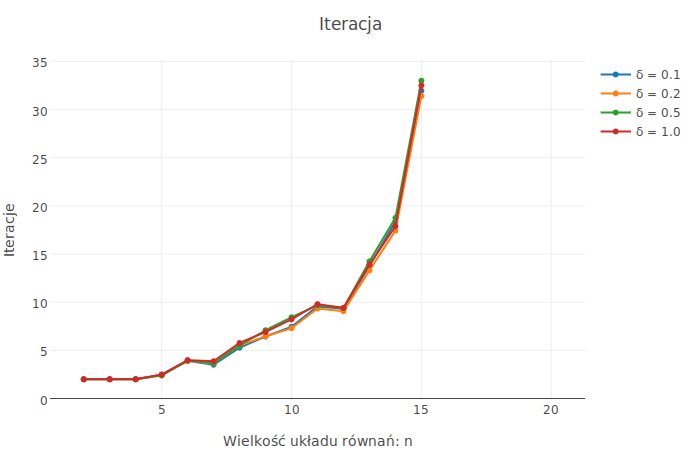
\includegraphics[width=0.9\textwidth]{avg_iterations_V}
    \caption{Średnia ilość iteracji potrzebna do zakończenia metody Newtona dla funkcji V \eqref{eq:V}}
    \label{fig:avgiterationsV}
\end{figure}
\begin{figure}[h]
    \centering
    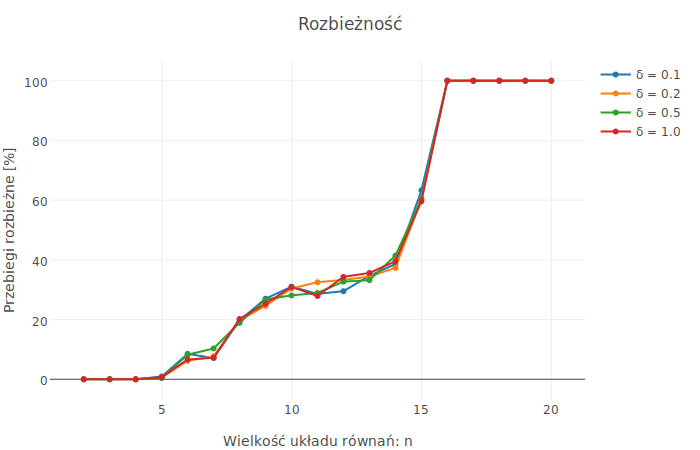
\includegraphics[width=0.9\textwidth]{avg_diversions_V}
    \caption{Procent uruchomień metody Newtona dla funkcji V \eqref{eq:V}, które nie zbiegły w limicie iteracji}
    \label{fig:avgdiversionsV}
\end{figure}
\FloatBarrier
\section{Analiza wyników}
Jak widać na wykresach \ref{fig:relprecision} oraz \ref{fig:norm} metoda Newtona dla funkcji wielu zmiennych nie zawsze jest zbieżna kwadratowo. Tak jak w przypadku funkcji jednej zmiennej, jeżeli pierwiastek którego szukamy jest wielokrotny lub pochodna zeruje się w pierwiastku, to nasz algorytm będzie zbieżny jedynie liniowo.

Dla badanych funkcji generujących duże układy można zaobserwować istotny wpływ przybliżenia początkowego na zbieżność algorytmu, co widać na wykresach \ref{fig:avgdiversionsF} i \ref{fig:avgdiversionsH}. Dla funkcjii $ F $ i $ H $ można także zaobserwować spadek zbieżności metody Newtona wraz z powiększaniem się układu równań (dla parametru $ \delta = 0.5, 1.0 $)

Zbieżność funkcji $ G $ jest natomiast nieczuła zarówno na wielkość układu, jak i przybliżenie początkowe, o ile jest ono względnie blisko $ \bar{x} $, tzn dla $ \delta \leq 0.5 $, co można zaobserwować na wykresie \ref{fig:avgdiversionsG}. Ta funkcja wykazuje także ciekawe zachowanie ilości iteracji względem wielkości układu. Z wykresu \ref{fig:avgiterationsG} widać, że dla $ \delta \leq 0.5 $ metoda Newtona osiąga maksimum potrzebnych iteracji dla $ n = 6 $, po czym ilość ta gwałtownie maleje i stabilizuje się.

Z wykresów \ref{fig:avgiterationsF} oraz \ref{fig:avgiterationsH} (dla $ \delta = 1.0 $ )  można natomiast wywnioskować, że ze wzrostem wielkości układu rośnie ilość iteracji potrzebna do znalezienia miejsca zerowego funkcji $ F $ oraz $ H $. Zarazem widać, że dla $ \delta \leq 0.5 $ obliczenie pierwiastka funkcji H wymaga praktycznie stałej ilości iteracji, niezależnie od wielkości układu.

Przy obliczaniu jakobianu funkcji $ V $ \eqref{eq:V} otrzymamy macierz Vandermonde'a, dla której metoda eliminacji Gaussa od pewnej wielkości macierzy generuje rozwiązania bardzo różne od prawdziwych. Efekt tego zachowania widać na wykresie \ref{fig:avgdiversionsV}, gdzie dla $ n \geq 16 $ metoda Newtona nie jest w stanie znaleźć rozwiązania. 

\section{Wnioski}

Na podstawie wykonanych obliczeń można stwierdzić, że metoda Newtona jest dość pewną metodą rozwiązywania układu równań nieliniowych, o ile potrafimy znaleźć dobre przybliżenie początkowe. Dla większości funkcji jest ona zbieżna kwadratowo. Największym problemem w wykorzystaniu tego algorytmu jest konieczność znania pochodnej funkcji $ F $ która dla dużego układu równań może być trudna do obliczenia. 

\begin{thebibliography}{99}

\bibitem{kincaid} David Kincaid, Ward Cheney, przekł.~Stefan Paszkowski,
\emph{Analiza numeryczna},
Warszawa, WNT, 2006.

\bibitem{ortega} J.~C.~Ortega, W.~C.~Rheinboldt,
\emph{Iterative Solution of Nonlinear Equations in Several Variables},
New York, Academy Press, 1970

\bibitem{bjorck} \r{A}ke Bj\"{o}rck, Germund Dahlquist, przekł.~Stefan Paszkowski
\emph{Metody Numeryczne},
Warszawa, PWN, 1987

\end{thebibliography}

\end{document}